\chapter{接口缺陷静态检测技术研究}
\label{cha:imchecker}
软件库通过应用编程接口(API)来封装已有功能,提高开发效率。
正确的接口使用需要满足特定的约束,否则引入接口误用,导致接口缺陷。
静态检测技术是在不运行程序的前提下对程序的行为进行分析的技术,
能够在开发早期进行应用,
极大地降低缺陷修复的成本。
现有的静态检测技术可以分为两类,基于程序分析的缺陷检测技术和基于数据挖掘的缺陷检测技术。
虽然现有工作能够对实际缺陷进行检测,然而存在若干不足。
主要表现在,(1)缺陷模式难以扩展,对用户自定义的接口支持不足;
(2)语义分析不足,检测结果不精确。
特别地,随着现代软件规模大、结构复杂,以及开源代码的广泛使用,使得检测技术面临新的挑战。
因此,研究精准高效的C程序接口缺陷检测技术,对于提升软件系统可靠性和安全性具有重要意义。

本章旨在研究规模化接口缺陷静态检测技术,以对大规模程序中接口误用缺陷进行准确、高效的检测,
弥补现有静态检测技术不足。
本章首先基于第\ref{cha:imchecker}章的缺陷模式对现有工作进行分析,总结现有工作的特点和不足。
接着提出了基于规约描述的规模化接口缺陷检测技术IMChecker。
IMChecker通过IMSpec规约描述以支持多种缺陷模式和用户自定义的接口,
基于多入口分析策略以应对实际项目中大规模代码,并基于语义信息和统计信息对结果的精度进行提升。
从全文的研究体系上看,
本章的工作是规约描述语言IMSpec的应用,同时是接口缺陷检测实际应用的重要核心。

\section{引言}
开发者在利用API快速构建系统的同时,需要满足接口使用时的约束条件,以正确执行接口内部封装的功能。
否则将会产生接口误用,导致软件缺陷。
对接口误用检测进行研究具有重要意义。
一方面,接口误用是导致软件错误、系统崩溃、漏洞产生的重要愿意之一。
CWE组织2011年发布的最危险的25个软件错误中,有40\%和接口误用相关~\cite{cwe-top25}。
同时,OWASP项目在2017年发布的最危险的10个网络漏洞中,有30\%和接口误用相关~\cite{owasp-top10}。
另一方面,随着开源社区的发展,软件库文档缺失、开发人员对API理解不足,
导致现有的代码中存在大量的接口误用缺陷。

近年来,研究人员设计并实现了各种各样的方法来检测接口缺陷。
特别地,静态检测技术获得广泛的关注和应用。
静态检测技术能够在不执行代码的情况下进行分析。
所以,可以应用于开发的各个阶段,有效的提高代码质量。
同时,静态分析在使用时不需要人工标记、构造测试用例和测试环境。
因此,能够对所有的程序路径进行模拟执行,使用范围广。
针对于接口缺陷检测,从分析策略上来说静态分析包含两种主要的技术路线:
程序分析技术~\cite{16-saner-evaluation}和数据挖掘技术~\cite{survey18}。
基于程序分析技术的检测方法和工具需要研究人员和工具实现者的领域知识,
通过规约描述或者程序硬编码的方式对目标接口使用的约束进行定义。
此后,基于程序语义,通过可达性分析、程序语义匹配等方式进行缺陷检测。
基于数据挖掘技术的方法和工具则通过统计学习的方法,根据算法设计者预定义的模式在项目中进行接口使用约束推理。
此后,基于推理的约束基于统计意义进行缺陷检测。

虽然,两者都能够在实际项目中进行应用并找到新的缺陷。
然而,两者存在两个主要不足:
(1)缺陷模式难以扩展,对用户自定义的接口支持不足。
前者无法应用于未定义的目标API,后者则依赖于大量高质量的数据以学习正确的约束。
(2)语义分析不足,分析精度不够,难以应用于实际项目中。
一方面,现有的工具多基于语法层分析;另一方面,为了支持大规模代码,
工具多在过程内分析,忽略了过程间的语义信息。


为解决上述方法中的不足,本章提出了基于规约描述的规模化接口缺陷静态检测方法IMChecker。
首先,IMChecker通过IMSpec规约描述以支持多种缺陷模式和用户自定义的接口。
精度和效率是静态分析技术需要平衡的重要指标。
高精度的分析技术需要昂贵的计算代价,从而限制了静态分析在实际项目上应用效果。
高效率的分析技术则存在分析精度的损失,产生大量的误报(False Positive, 将正确行为报告称缺陷)
和漏报(False Negative,实际缺陷没有被检测出)。
因此,基于多入口分析策略,将复杂的程序分析问题分而治之,高效率分析的同时,
实现局部的精确分析。
针对于多入口分析策略导致的分析精度的损失,
IMChecker通过基于上下文的语义摘要信息和基于使用情况的统计信息进行结果过滤,
以提交检测的精度。
本章基于目前已知最大规模的开源缺陷测试集Juliet Test Suite中,13个接口缺陷相关的CWE分类对IMChecker方法进行评估。
实验结果显示,IMCHecker方法误报率为13.21\%,漏报率为16.08\%。
检测能力领先于主流的开源软件项目。

本章其余部分组织结构如下:
\ref{sec:3.2}节对相关研究进行总结;
\ref{sec:3.3}节对规模化接口缺陷静态检测算法进行介绍;
\ref{sec:3.4}节给出工具评估和研究评估结果;
最后在\ref{sec:3.5}节总结本章工作。
\section{相关工作}
\label{sec:3.2}

静态缺陷检测方法在不执行程序的情况下,对程序中的缺陷进行检测。
针对于C程序接口缺陷,近年来,研究人员和工具开发者设计并实现了各种各样的静态检测算法和工具~\cite{16-saner-evaluation, survey18}。
本节对其中的典型算法和工具进行调研和总结。

从技术路线上来说,静态缺陷检测方法可以分为两大类,
\begin{itemize}
	\item {\kaishu 程序分析技术}程序分析技术需要明确的提供目标接口的使用约束。
	因此需要研究人员和开发者具有良好的领域知识。
	目前,约束的描述方式有两种:规约描述语言和程序硬编码检测器。
	前者在分析的过程中,首先将语言进行解析并构造监控自动机的中间表达。
	在程序语义分析阶段,通过可达性分析对缺陷进行检测。
	该方法有利于对新的接口进行扩展,即提供对应的缺陷描述。
	后者则在分析的过程中,基于程序语义进行模式匹配对缺陷进行检测。
	该方法难以扩展,需要实现新的检测器。
	基于程序分析技术的工作,最大的优点是可以有效利用积累的领域知识,以及利用语义分析获得更加准确的分析结果。
	\item {\kaishu 数据挖掘技术}数据挖掘技术则不需要用户提供显示的约束,
	可以基于统计信息,基于学习的方法自动推理约束。
	其检测的核心在于,通过对程序形式的转化,构造中间表达。
	并基于预先定义的模式,基于统计信息学习接口使用的约束。
	特别地,大多数方法认为:多数使用为正确用法,少数为错误。
	虽然基于数据挖掘技术的检测方法不要人定义具体的约束,
	但是需要良好领域知识设计学习模型。
	因此,其扩展性交叉。
	基于数据挖掘技术的工作,最大的优点是设计好学习模型后可以实现完全自动化,同时不需要项目特定的领域知识。
\end{itemize}

具体来说,如表~\ref{tab:3-2-survey}中所示,本文共对17个研究工作和工具进行调研的总结。
其中前五个为基于程序分析技术的普适性静态缺陷检测工具,包括开源软件三个,以及两个商业工具的学术使用版。
第6-7个为针对接口设计的基于程序分析技术的静态缺陷检测工具。
最后10个则为基于数据挖掘技术的程序接口缺陷检测技术。
针对于提供工具的工作,作者对工具进行使用;
对于没有工具的工作,作者对论文进行阅读,总结其检测能力。
特别地,为了减少作者的主观臆断带来的影响。
对于每一个工作,作者或直接和论文作者进行结果核对,或同时阅读了3-5个引用该论文的其他工作,与这些论文中的描述进行核对。

\begin{table}[t]
	\centering
	\begin{minipage}[t]{0.85\linewidth} % 如果想在表格中使用脚注,minipage是个不错的办法
		\caption{静态分析工具对C程序接口缺陷检测能力}
		\label{tab:3-2-survey}
			\begin{tabular}{@{\extracolsep{3pt}}ccccccccccc@{}}
			%\begin{tabular}{ccccccccccc}
			\hline
			\multirow{2}{*}{工具名称} & \multicolumn{2}{c}{IPU\footnote{Y:支持,P:部分支持,-:不支持}} & \multicolumn{3}{c}{IEH} & \multicolumn{3}{c}{ICC} & \multirow{2}{*}{扩展性\footnote{难:难以扩展,有限:可以扩展,扩展内容受限,-:不支持,$\checkmark$:方便扩展}} & \multirow{2}{*}{可用性\footnote{$\checkmark$:可用且基本符合预期,P:可用但与预期相差很大,-:不可用}} \\
			\cline{2-3}\cline{4-6}\cline{7-9}
			 & -s & -r & -c & -p & -l & -s & -c & -r & & \\
			\hline
			Clang-SA~\cite{clang-sa} & Y & Y & - & - & - & Y & Y & Y & 难 & $\checkmark$ \\
			Cppcheck~\cite{cppcheck} & Y & Y & P & - & P & Y & Y & Y & 有限 & $\checkmark$ \\
			Infer~\cite{infer} & Y & Y & - & - & - & Y & Y & Y & - & $\checkmark$ \\
			Pinpoint~\cite{pinpoint} & Y & Y & P & - & - & Y & Y & Y & - & $\checkmark$ \\
			Coverity~\cite{coverity} & Y & Y & Y & P & P & Y & Y & Y & 难 & $\checkmark$ \\
			\hline 
			SLAM~\cite{slam} & Y & Y & Y & - & - & Y & Y & Y & 有限 & $\checkmark$ \\
			SSLINT~\cite{15-sp-sslint} & P & - & Y & - & - & Y & Y & - & 有限 & - \\
			\hline
			PR-Miner~\cite{05-fse-prminer} & - & - & - & - & - & Y & Y & - & - & - \\
			RGJ07~\cite{07-PLDI-RGJ07} & Y & Y & - & - & - & Y & Y & - & - & - \\
			Chronicler~\cite{07-icse-chronicler} & - & - & - & - & - & Y & P & - & - & - \\
			EDP~\cite{08-fast-eio} & - & - & Y & Y & - & - & - & - & - & - \\
			Hector~\cite{13-dsn-hector} & - & - & - & - & - & Y & P & - & - & - \\
			Chucky~\cite{13-ccs-chucky} & P & P & Y & - & - & - & - & P &  & \checkmark \\
			NDNR14~\cite{14-fse-pre} & P & Y & - & - & - & - & - & - & - & - \\
			APISan~\cite{16-sec-apisan} & P & P & Y & Y & - & Y & Y & P & - & \checkmark \\
			Antminer~\cite{16-icse-antminer}& P & P & Y & P & - & P & P & - & - & - \\
			ErrDoc~\cite{17-fse-errdoc}& - & - & Y & Y & P & P & - & - & 有限 & P \\
			\hline
		\end{tabular}
	\end{minipage}
\end{table}
如表~\ref{tab:3-2-survey}中所示,本文从三个方面共对17个研究工作和工具进行调研的总结。
即,检测能力、扩展性和可用性。
表中第一列为项目名称。
第2-9列,为工具对于第~\ref{sec:2.3}节中总结实际项目的缺陷模式的支持情况。
特别地,IPU-s代表单个参数的检查、IPU-r代表参数之间和参数与返回值之间的检测;
IEH-c代表异常处理中对接口返回值的检测、IEH-p为异常处理中返回错误代码的检测(error propagation)、
IEH-l为异常处理中对缺陷信息打印支持的检查;
ICC-s为不带上下文关系的接口对、ICC-c为带有上下文关系的接口对、ICC-r代表重复调用的检测。
第10列扩展性关注,算法和工具是否能够针对用户需求预留了扩展的接口,对项目特定的接口检测进行扩展。
其中难表示可以扩展,但是代价非常大,比如Clang-SA需要重新设计检查器插件;
有限代表工具提供了扩展的方式,但是扩展的内容需要满足特定的缺陷模式。
最后一列为工具的可用性,即该工具是否可用。
特别地,工具的效果是否和发表的论文、工具说明一致。
其中,P代表工具可以下载和使用,但是其功能和论文描述不符。
即,工具难以支持论文中明确给出的代码样例。

检测能力方面,
从表中调研结果可知,在所有的工作中,并没有一个工作能够完全的支持所有的接口缺陷模式。
特别地绝大多数基于数据挖掘技术的工作,只能处理某一种特殊的缺陷模式。
检测能力最好的是商业工具Coverity和基于数据挖掘技术的工具APISan。
然而前者实际价格昂贵,难以广泛使用。
后者基于数据挖掘技术,工具作者在论文中指出,具有极高的误报率。
此外,在所有缺陷模式中,单个参数检查、异常处理中返回值检查和
不带有上下文语义关系的函数调用对检查被大多数工具支持。
这些缺陷模式相对简单,能够从语法结构直接进行检查。
然而,本文作者发现,绝大部分工具并没有考虑足够的语义信息。
例如,对于参数的检查,如果缺少参数或者代码中参数与常量比较则工具支持效果较好。
但是如果比较的方式为和变量比较,则工具存在大量漏报。

扩展性方面,只有6个工具提供了扩展的接口。
其中Clang-SA和Coverity需要设计新的检测器插件,扩展难度极大。
SLAM、SSLINT、Errdoc可以通过撰写规约的方式对检测目标扩展,然而其只能针对于特定的缺陷模式或者项目特定的接口扩展。
即SLAM针对于Windows操作系统内核的驱动程序设计,SSLINT针对于SSL/TLS安全协议设计和
Errdoc针对于异常处理设计。
Cppcheck为用户提供了最方便的扩展接口。
通过提供结构化的接受使用描述方式,用户可以对自定义的接口进行扩展。
然而,Cppcheck提供的语言只能够支持单个参数、参数关系、返回值检测和不带因果关系的函数对四种情况。

应用性方面,基于数据挖掘的工作中可用的工具只有Chucky和APISan。
Errdoc工具在适用时,作者发现其与论文描述差距较大。
基于程序分析技术的工具作者选择的都是可以使用工具,因此实用性较好。
然而,在实际项目应用中,作者发现,这些工具的分析报告存在两种极端的表现。
即要么报告数量多,但存在大量的误报;要么报告数极少,与其他工具项目,存在大量的漏报。

总体来说,针对于C程序接口缺陷检测,现有的工作存在两点主要不足。
(1)缺陷模式支持有限,扩展性不足,难以支持用户自定义的接口。
一方面,基于程序分析的技术需要通过规约撰写或者开发新的检测插件。
如第~\ref{sec:2.2}和本章调研结果所示,现有的约束描述方法或过于复杂,或难以扩展到全部接口缺陷模式。
同时,开发新的插件则需要理解工具框架和细节,难以实际使用。
另一方面,基于数据挖掘的技术需要大量可靠数据进行约束学习。
然而,该需求对于独立的项目难以实现。特别地,用户自定义的接口往往使用次数有限,
难以满足学习所需要的数据量。
(2)语义分析不足,检测结果存在大量误报和漏报,难以支持实际项目分析。
一方面,为了提高缺陷检测的效率,现有的工具多基于语法结构对缺陷分析。
因此,难以支持需要语义信息的缺陷。
另一方面,多数工具基于过程内分析策略,以应对大规模程序。
然而,丢失的上下文语义信息,会导致误报和漏报。

\section{接口缺陷静态检测算法}
\label{sec:3.3}
本节提出IMChecker,以解决上述不足。
通过 1 2 3 来做什么


(seke19)
我们以图1.1中的例子作为案例,

介绍总体图和流程

每部分的主要工作
1.5页

\subsection{构造分析上下文}
编译抓取,为什么IR

介绍CFA,给一个图
1页

对于命令式语言的程序可以用控制流自动机(Control-flow Automaton,CFA) cxP3.3.1

多入口分析策略cx89
0.5页

函数展开
循环
0.5

\subsection{抽象符号路径提取}
语法

解释用例子

结果
1.5页
\subsection{缺陷检测算法}
算法
1页
例子解释
0.5页

%\begin{algorithm}
	\KwIn{~~~\textsf{SyncBlock} 计算模型内所有复合构件的 $<connection>$,
		\\~~~~~~~~~~~~~~~顶层复合构件的所有输入端口 $<port\_declaration>$,
		\\~~~~~~~~~~~~~~~顶层的每一个输入端口 $p_i$ 对应的环境输入值 $I_i$。 }
	\KwOut{更新所有与顶层复合构件输入端口相连接的端口的值。}
	\vspace{3ex}
	%\SetAlgoLined
	\For{~~顶层复合构件 $<port\_declaration>$ 中的每一个输入端口 $p_i$~~}{
		$p_i \gets I_i$ \;
		\tcp{取出所有与 $p_i$ 直接相连的内部子构件的端口}
		$p_i \left[\right] \gets Connection\_Target(p_i,~<connection>)$ \;
		\For{~~$p_i \left[\right]$ 中的每个端口 $p_i\left[ j \right]$~~} {
			\tcp{根据端口 $p_i\left[ j \right]$ 的性质,判断是否要继续向下搜索传递}
			\eIf{~~$p_i\left[ j \right]$ 不是原子构件的输入端口~~}{
				\tcp{如果连接上有表达式,进行数据处理再赋值}
				\eIf{~~$<connection>$~上有表达式~~}{
					$p_i\left[ j \right] \gets Comput\_Exp(p_i)$ \;
				}{
					$p_i\left[ j \right] \gets p_i$ \;
				}
				\tcp{取出所有与$p_i\left[ j \right]$ 直接相连的端口,添加到 $p_i \left[\right]$ 中}
				$p_{temp} \left[\right] \gets Connection\_Target(p_i\left[ j \right], <connection>)$ \;
				$p_i \left[\right] \gets Append(p_i \left[\right], p_{temp} \left[\right])$ \;
				
			}{
				\tcp{$p_i\left[ j \right]$ 是原子构件的输入端口,不需要继续向下搜索传递}
				\eIf{~~$<connection>$~上有表达式~~}{
					$p_i\left[ j \right] \gets Comput\_Exp(p_i)$ \;
				}{
					$p_i\left[ j \right] \gets p_i$ \;
				}
			}
			
		}
	}
	\caption{从外部环境读入输入序列,传递到原子构件输入端口}
	\label{alg:Input}
\end{algorithm}


\subsection{检测结果过滤}
为什么

语义例子

统计例子
1.5页
\section{工具实现与实验评估}
\label{sec:3.4}
本节首先介绍规模化接口缺陷检测方法IMChecker的实现细节。
随后在公开数据集上,对IMChecker的分析能力进行评估,并给出IMChecker与主流开源工具的比较结果。

\begin{figure}[t]
	\centering
	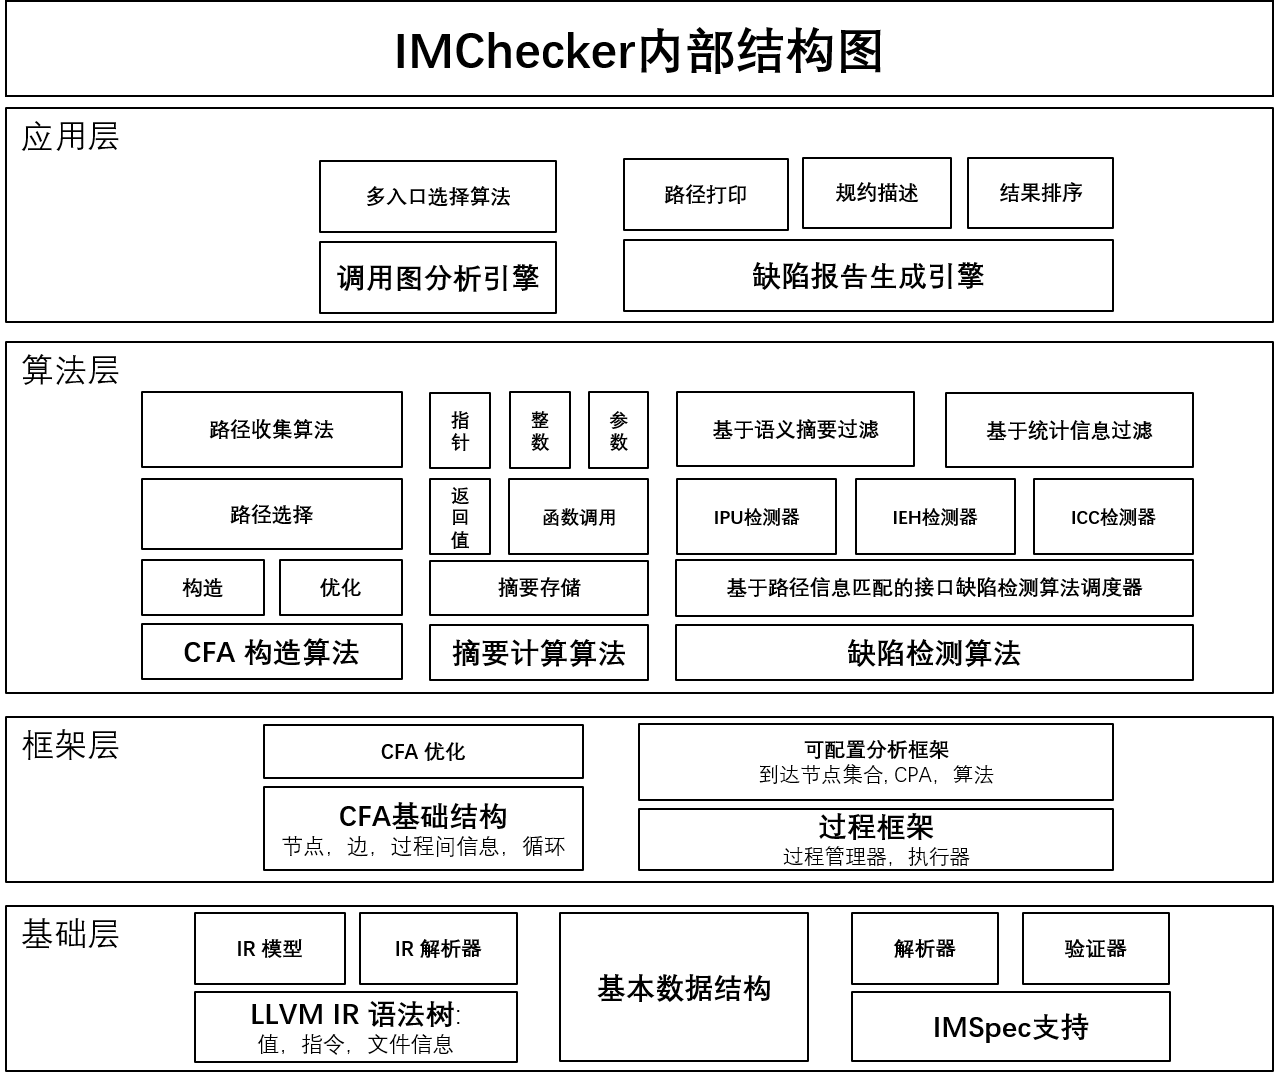
\includegraphics[width=0.9\linewidth]{figures/cp3-implementation.png}
	\caption{
		IMChecker工具内部结构图
	}
	\label{fig:3-4-implementation}
\end{figure}

\subsection{工具实现}
IMChecker基于Java语言实现,依赖于LLVM3.9的IR作为分析的中间表达,
并基于CPA~\cite{07-cav-cpachecker}算法作为整体方法的实现基础。
工具接口用户提供的源代码和IMSpec规约描述作为输入。
其中IMSpec实例和缺陷检测结果都基于Yaml~\cite{yaml}格式存储。
工具实现的内部结构如图~\ref{fig:3-4-implementation}所示。
工具共包含四个层次:基础层、架构层、算法层和应用层。
首先,基础层通过对源代码处理,生成LLVM-IR中间表达;并对IMSpec规约描述进行解析和一致性分析。
架构层构造CFA,将程序转化为图结构;
同时,提供基于CPA算法的分析流程以支持上层语义计算的算法。
算法层,则对CFA进行优化、计算语义摘要信息以及缺陷检测。
最后,应用层通过调用图具体进行分析入口的选择,执行缺陷分析;
并将缺陷检测的结果进行过滤、排序和信息打印。

\paragraph{基础层}
基础层旨在对用于输入的源代码和IMSpec规约描述进行预处理,同时提供分析中需要的基本数据机构。
首先,针对于用户输入的源代码,
如果待测程序是单个的C文件,IMChecker直接使用clang编译器
\begin{lstlisting}[language={bash},
basicstyle=\linespread{0.8}\listingsfont,
numbers=none,
xleftmargin=.25\textwidth]
(*@\textcolor{blue}{Ubuntu@~: clang}@*) path2source -S -emit-llvm -g
\end{lstlisting}
进行预处理以生成自包含的.ll文件。
该文件相比于原.c文件增加了必需的函数和数据结构声明,展开了宏定义,消去了预处理指令等。
同时生成了对应的LLVM-IR中间表达。
如果待测程序是一个Makefile工程,
那么通过解析Makefile中的编译指令并且将所有输出.o文件的指令替换为相应的预处理指令,例如clang -E。
预处理生成的.i文件,再利用上述指令生成.ll文件。
同时,根据Makefile的编译目标,项目被组织成不同的分析任务。
通过llvm的链接指令(llvm-link)将给定分析任务下所有的.ll文件进行合并,
作为输入进行缺陷检测。
在获得LLVM-IR中间表达后,利用javacpp\footnote{https://github.com/bytedeco/javacpp}工具解析文件,
并构造IR模型,包括值、指令和文件信息。
另一方面,基础层对用户提供的IMSpec语言进行解析。
IMSpec语言针对于单个目标API设计,所以如果规约中存在语法错误则将错误规约忽略并输出给使用者。
同时,解析后的IMSpec进行语义一致性验证,即是否存在冲突的约束。
例如,一个条件未接口的第一个参数大于零,另一个条件未第一个参数小于零等等。

\paragraph{框架层}
框架层旨在提供分析框架的实现以及基本土结构的创建。
在对用户提供的源代码解析过后,CFA基本结构模块对LLVM-IR进行包装,构造CFA结构。
特别地,CFA在节点上表示程序的位置,在边上封装程序的具体执行指令。
为了在CFA图上提供更多的语义信息,
本文将CFA边分为两种,即控制边和摘要边。
前者表示具体的语义操作的指令,例如存储、运算、返回等等。
后者表示函数调用和循环关系。
因此,通过摘要边,在分析中可以利用摘要信息跳过函数展开和循环遍历,
在保证大规模代码有效分析的同时增加分析精度。
IMChecker基于过程(Phase)来运行,即每个过程复杂不同的预处理或者检测步骤。
所以,框架层中实现了过程管理的调度器。
特别地,IMChecker基于CPA算法来实现具体的路径抽取和缺陷检测。
因此IMChecker在框架层实现了CPA算法的核心数据结构和基础调度算法。
具体的每一个CPA则在算法层中实现。

\paragraph{算法层}
算法层旨在实现具体的算法细节。
IMChecker针对C程序接口使用缺陷进行检测,在整个分析过程中可以分为三个阶段:
路径收集、摘要计算和缺陷检测。
\begin{itemize}
	\item {\kaishu 路径收集} 在路径收集阶段,IMChecker利用CFA构造算法,对框架层的CFA原型进行优化。
	特别地,为了支持大规模程序分析,IMChecker基于入口分析。
	因此,在这个阶段对入口进行标记。
	此后,基于优化后的CFA图结构,通过第~\ref{sec:3.3}节中的路径抽取方法,
	收集路径信息,为后续两个步骤做准备。
	目前IMChecker基于AccesPath~\cite{15-ase-accesspath}和整数分析对语义信息进行计算。
	\item {\kaishu 摘要计算} 
	摘要计算的结果应用于缺陷检测当中,在实现上,IMChecker则先进行摘要的计算。
	为了支持大规模程序检测,IMChecker采用了基于多入口分析的策略,使得分析精度下降,
	导致大量误报。
	为了提供更加准确的检测结果,IMCHecker利用上下文语义信息对结果进行过滤。
	具体而言,IMChecker计算:上下文指针常量计算、整数常量计算、参数约束关系、
	返回值常量关系和函数调用关系的摘要信息。
	\item {\kaishu 缺陷检测} 
	缺陷检测部分,IMChecker实现了基于路径信息匹配的接口缺陷检测算法。
	特别地,为了提高检测精度,IMChecker实现了检测算法调度器。
	即,根据使用约束的不同,调用不同的检测算法的实现,以精确分析程序进行缺陷检测。
	最后,利用基于语义的摘要信息和基于使用情况的统计信息对结果过滤。
\end{itemize}


\paragraph{应用层}
应用层旨在从方法实际程序运行的角度,对IMChecker进行封装和优化。
一方面,应用层实现了多入口选择算法和调度引擎。
通过该模块,具体执行每个入口的分析。
另一方面,对于检测后的缺陷,生成相应的缺陷报告。
包括,缺陷产生的路径信息、违反的规约描述和具体约束条件的IMSpec形式和自然语言解释。
特别地,IMChecker基于使用情况对缺陷检测结果进行排序。
目前,在满足最低使用次数(Minimum Support)的情况下,
IMChecker认为误用次数与使用次数的比例越小(Confidence)。
即该缺陷与大多数使用不一致,则该检测结果越有可能是缺陷。

IMChecker已经集成在Tsmart工具集中~\cite{tsmart},工具使用的具体细节将在第~\ref{sec:4.3}中进行介绍。

\subsection{实验准备}

\paragraph{测试集} 由于目前并没有针对C程序接口缺陷检测的测试集合,
因此作者基于美国国家标准技术研究所(NIST) 整理的Juliet Test Suite测试集~\cite{juliet},
对IMChecker的分析能力进行评估。
该测试集合包含超过6万个C/C++用例,涵盖118个不同的CWE缺陷类型,
是目前最为广泛使用的测试集。
本文根据接口缺陷模式共选取了13个具体的分类。
Juliet测试集合每个分类中给出了大量的重复模式的测试用例,和不同的产生原因。
因此,作者对其中重复的用例进行过滤,保留由于接口误用导致错误的测试用例。
同时,对每个分类中的缺陷实例进行过滤和修正,
以确保其函数至少一个误用和一个修复后的版本。
如表~\ref{tab:3-4-cwe}所示,针对于第~\ref{sec:2.3}中总结的三大类接口误用模式,
共选取了2172个测试用例。
为了方便研究人员和开发者理解缺陷模式和评估检测工具,
本文将这些修订后的测试用例集成到APIMU4C,C程序接口误用数据集中。
APIMU4C将在第~\ref{sec:4.2}详细介绍。


\begin{table}[t]
	\centering
	\begin{minipage}[t]{0.8\linewidth} % 如果想在表格中使用脚注,minipage是个不错的办法
		\caption{评估测试集组成}
		\label{tab:3-4-cwe}
		\begin{tabular}{cccl}
			\hline
			{缺陷类别 } & {CWEID} & 缺陷数目 & \multicolumn{1}{c}{缺陷描述} \\
			\hline
			\multirow{6}{*}{IPU} & 121 & 36 & 栈内存越界读取\\
			& 122 & 36 & 堆内存越界读取 \\
			& 131 & 42 & 不正确的计算缓冲区大小\\
			& 476 & 36 & 空指针引用\\
			& 590 & 360 & 释放非堆内存\\
			\cline{2-4} 
			& \multicolumn{3}{c}{5个CWE分类,510个测试用例} \\
			\hline
			\multirow{3}{*}{IEH} & 252 & 270 & 未检查错误状态代码\\
			& 253 & 270 & 错误状态代码检查不正确\\
			& 390 & 72 & 未进行异常处理\\
			\cline{2-4} 
			& \multicolumn{3}{c}{3个CWE分类,612个测试用例} \\
			\hline
			\multirow{5}{*}{ICC} & 401 & 474 & 内存泄漏\\
			& 404 & 24 & 不正确的资源释放\\
			& 415 & 120 & 重复释放\\
			& 690 & 384 & 未对因果调用中的上下文关系检测\\
			& 775 & 48 & 未释放文件资源\\
			\cline{2-4} 
			& \multicolumn{3}{c}{5个CWE分类,1050个测试用例} \\
			\hline
		\end{tabular}
	\end{minipage}
\end{table}

\paragraph{ 比较对象}
首先,为了检测过滤机制的效果,本文将未添加过滤机制的方法记作为IMChecker--。
通过IMChecker与IMChecker--在测试集上的表现差别,以评估过滤算法的有效性。
此外,本文选取广泛使用的代表性开源工具进行检测能力的比较。
在对工具描述文档、学术论文和预实验后,本文选取了如下三个工具:
\begin{itemize}
	\item APISan~\cite{16-sec-apisan}(主分支-2018-0601):
	该工具是一个开源的学术工具,针对于接口误用缺陷设计。
	通过数据挖掘技术与程序分析技术结合,利用轻量级语义分析方法获得接口使用上下文信息,
	并基于统计方法推理接口使用约束。
	工具基于过程内分析方法,考虑函数返回值、参数关系和因果调用关系,并将规约推理的结果用于缺陷检测。
	不过,推理的结果没有输出,也没有提供扩展规约推理方法或者接受约束的接口。
	\item Cppcheck~\cite{cppcheck}(版本1.83):
	Cppcheck是针对于未定义和危险程序结构的缺陷检测工具。
	该工具开源代码,并支持多个领域和不同的缺陷类型。
	将代码转化为字节流(token)后,
	基于上下文敏感(context-sensitive)和流敏感(flow-sensitive)的过程间分析方法,
	对缺陷进行模式匹配。
	Cppcheck在检测算法中集成了C标准库的接口。
	同时,为了支持用户自定义的接口,提供了一套规约描述方法\footnote{http://cppcheck.sourceforge.net/manual.pdf, chapter10, page 20.},以利用实现过算法对相同的缺陷模式进行检测。
	例如参数空指针,内存泄漏等等。
	\item Clang-SA~\cite{clang-sa}(版本RELEASE\_600):
	该工具是LLVM开源编译器的组成部分。
	通过符号执行技术,推理程序语义。
	该工具采用上下文敏感(context-sensitive)和流敏感(flow-sensitive)的过程间分析方法,
	并实现了大量的检测插件,以应对不同的缺陷类型\footnote{http://clang-analyzer.llvm.org/available checks.html}。
\end{itemize} 
一方面,这三个工具提供了良好的缺陷报告接口,支持多种接口缺陷类型。
另一方面,这三个工具基于不同的分析技术(数据挖掘、静态分析-硬编码、静态分析-基于规约描述)。
同时,三个工具在预实验中的检测能力稳定,与文档论文中的描述能力一致。

\paragraph{评测指标}
在测试集上,本文将采用如下三个指标对工具进行评估。
\begin{itemize}
	\item 召回率(Recall):$R = \dfrac{\text{结果报告中真实的缺陷数}}{\text{总缺陷数}}$
	召回率是基于具体实现情况下,工具的检测能力。即,工具能够有效的检测多少缺陷。
	缺陷检测领域普遍认为,一个工具在测试集合上的召回率越高,那么其实际应用中也会有更好的检测效果。
	\item 精度(Precision):$P = \dfrac{\text{结果报告中真实的缺陷数}}{\text{工具报告的缺陷总数}}$
	研究表明,困扰实际用户使用静态分析的原因之一就是,现有的工具产生了大量的误报,即精度太低~\cite{10-acm-precision}。因此,检测工具的精度是重要的指标之一。
	特别地,如果精度低于30\%,那么实际使用者将抛弃这个工具。
\end{itemize}
%\item 理想召回率(Conceptual Recall,CR):$= \dfrac{理想情况下能够支持的缺陷数}{工具报告的缺陷总数}$
%该指标表示工具能够支持的最大程序的检测能力。即,工具用户手册或者论文中,不考虑实现的正确性下,提到能够解决问题的全部空间。一个工具的CR越高,代表这个工具的检测能力越强。 $R = \frac{结果报告中真实的缺陷数}{总缺陷数}$

\paragraph{运行环境} 本文在一台装有64 位Ubuntu 16.04的台式机上进行实验。
该机器配有Intel(R) Core(R) i5-3470@3.20GHz-4核心CPU和32GB内存。
本章关注接口缺陷检测的能力,因此不设置最长分析时间。


\subsection{评测结果}

\begin{table}[b]
	\centering
	\begin{minipage}[t]{0.9\linewidth} % 如果想在表格中使用脚注,minipage是个不错的办法
		\caption{IMChecker评测结果}
		\label{tab:3-4-imchecker}
		\begin{tabular}{cccccccccc}
			\hline
			\multirow{2}{*}{类别 } & \multirow{2}{*}{个数} & \multicolumn{4}{c}{IMChecker} & \multicolumn{4}{c}{IMChecker-~-} \\
			\cline{3-10}
			 & & 报告数 & TP\footnote{TP:真实缺陷数目} & P(\%) & R(\%) & 报告数 & TP& P(\%) & R(\%) \\
			 \hline
			 IPU & 510 & 490 & 423 & 86.33 & 82.94 & 745 & 469 & 62.95 & 91.96 \\
			 IEH & 612 & 580 & 506 & 87.24 & 82.68 & 677 & 526 & 77.70 & 85.94 \\
			 ICC & 1050 & 1012 & 878 & 86.76 & 83.62 & 1320 & 898 & 68.03 & 85.52 \\
			 总计 & 2172 &  2082 & 1807 & 86.79 & 83.20 & 2742 & 1893 & 69.04 & 87.15 \\
			\hline
		\end{tabular}
	\end{minipage}
\end{table}
\paragraph{IMChecker评测结果}
评测结果如表~\ref{tab:3-4-imchecker}中所示,
其中报告数为工具缺陷的总报告数,TP为报告中真实存在的缺陷数目,P为精度,R为召回率。
表中3-6列为IMChecker的评估结果,7-10列为IMChecker--的评测结果,即不包括过滤机制的结果。

评测结果表明,在所有的测试用例中,
IMChecker--共产生2742个缺陷报告,其中1893个为真实的缺陷,
849个为误报,平均精度为69.04\%,平均召回率为87.15\%。
在对缺陷报告深入分析后,导致IMChecker--分析结果不准确的主要原因是跨函数的接口使用。
如第~\ref{sec:3.3}中所示,为了能够支持大规模代码有效分析,IMChecker的检测算法基于过程内分析进行。
因此,当接口使用跨函数时,则会导致分析精度下降。

我们通过\texttt{malloc/free}例子进行分析。
在C的标准库中,两者组合进行堆内存的申请和释放。
其使用约束是当前者的返回值不为NULL时,需要调用后者进行释放。
然而IMChecker基于过程内的分析方式,对于跨越函数调用的接口,分析精度不足。
一方面,语义信息的不足会产生误报,即将正确的用法报告称缺陷。
例如下面代码所示,
\begin{lstlisting}[language={C},
basicstyle=\linespread{0.7}\listingsfont,
numbers=left,
xleftmargin=.2\textwidth]
void bar(int* p){
	// do
	free(p);
}
void foo(){
	int* p = (int*) malloc(100*sizeof(int));
	if (p == NULL) return;
	bar(p);
}
\end{lstlisting}
IMChecker--在第6行发现调用了\texttt{malloc}函数,在第7行对返回值进行检测,
需要调用\texttt{free}函数进行内存释放。
然而该释放操作在第3行的\texttt{bar}函数内进行,
因此IMChecker--并没有捕获这样的信息,导致将该用例判断为缺陷,产生一个误报。
另一方面,同样的语义信息不足则可能导致漏报,即没有检测到缺陷。
\begin{lstlisting}[language={C},
basicstyle=\linespread{0.7}\listingsfont,
numbers=left,
xleftmargin=.2\textwidth]
void bar(int* p){
	// do
	free(p);
}
void foo(){
	int* p = (int*) malloc(100*sizeof(int));
	if (p == NULL) return;
	bar(p);
	free(p);
}
\end{lstlisting}
例如上述代码所示,IMChecker--在第9行检测到\texttt{free}函数。
同时该函数的参数与\texttt{malloc}的返回值指向同一块内存。
因此,IMChecker--会将该用例判断为缺陷。
然而,在\texttt{bar}函数内,已经对该指针所指向的内存释放。
所以这是一个重复释放内存错误(CWE-590)。

为了解决上述问题,提高检测的精度,消除跨函数语义带来的影响。
如第~\ref{sec:3.3}节介绍,IMChecker引入了基于语义和基于使用情况的过滤机制。
在结合过滤算法后,IMChecker共产生2082个缺陷报告,其中1807个为真实缺陷。
IMChecker的平均精度为86.79\%,平均召回率为83.20\%。
相比较于IMChecker--,在有限的召回率损失下(3.95\%),
IMChecker检测精度有了显著提高(17.75\%)。
损失的召回率由于过滤机制中,对于参数和返回值的处理造成。
\begin{lstlisting}[language={C},
basicstyle=\linespread{0.7}\listingsfont,
numbers=left,
xleftmargin=.2\textwidth]
void foo(int **p) {
	*p = (int*) malloc(100*sizeof(int));
	// do
}
\end{lstlisting}
在实际项目中,我们发现大量的内存申请结果赋值给参数或者返回值。
并在外界进行检测和维护。
因此,IMChecker将这种情况下的缺陷过滤。
然而如果外界缺少必要的操作,则会产生漏报。
同时,虽然引入了过滤机制,IMChecker依旧存在误报和漏报。
目前,IMChecker基于语义的过滤机制目前只计算一层函数调用的摘要信息。
因此,当调用信息超过两层时,依旧无法准确检测。
例如如下代码片段,
\begin{lstlisting}[language={C},
basicstyle=\linespread{0.7}\listingsfont,
numbers=left,
xleftmargin=.2\textwidth]
void bar1(int* p){        
	// do						   
	free(p);					  
}
void bar1(int* p){        
	// do						   
	bar2(p);					  
}
void foo(){...}
\end{lstlisting}
由于释放函数跨越两层调用,因此无法被过滤,IMChecker将产生一个误报。


此外其他一些原因同样导致IMChecker分析不够精确,包括:
\begin{itemize}
	\item 复杂的数据依赖关系。
	目前IMChecker基于CPA算法实现,通过AccessPath的方式记录指向关系并维护整数信息。
	然而当,指针存在偏移操作时,如果偏移的位置不为常量,那么IMChecker就会认为这个指针指向该内存对象所有的区间。
	另一方面,由于目前只维护了常量整数。因此,当整数为变量时,IMChecker会认为该值可能为任何值。
	例如,\texttt{memcpy(d,s,n)}拷贝内存内容。拷贝的长度n应小于目标d的大小。
	然而当程序中,无法对n和d的关系进行推理时,IMChecker则会认为是错误,从而产生误报。
	\item 函数指针。C程序提供了函数指针的语言特性。因此,在静态分析阶段,无法明确或者该指针的指向关系。
	IMChecker在分析的过程中会忽略这部分内容。导致误报和漏报。
	\item 循环。循环问题在程序分析中是至今无法很好解决的难题。
	特别地,针对于接口缺陷,如第~\ref{sec:3.3}节介绍,缺陷实例调研结果显示,
	接口缺陷很少发生在循环汇总。因此,IMChecker只展开一次循环。
	对于如下代码中的重复释放问题,IMChecker则会产生漏报。
\begin{lstlisting}[language={C},
basicstyle=\linespread{0.7}\listingsfont,
numbers=left,
xleftmargin=.2\textwidth]
	char * data;
	data = NULL;
	for(i = 0; i < 1; i++){
		data = (char *)malloc(100*sizeof(char));
		strcpy(data, "A String");
	}
	for(k = 0; k < 2; k++){
		free(data);
	}
\end{lstlisting}	
\end{itemize}

针对于上述总结的不足,一个可行的解决方案引入更加精确的分析方法。
例如,增加跨函数分析、增加循环展开、增加函数指针的映射关系、利用更精确的值分析方法等等。
然而这些精确的语义计算会极大地影响分析效率。
因此,如何平衡分析效率与精度需要更多的尝试。
本文将在第~\ref{cha:con}章中进行描述。

\paragraph{IMChecker与其他工具对比结果}

\begin{table}[b]
	\centering
	\begin{minipage}[t]{0.9\linewidth} % 如果想在表格中使用脚注,minipage是个不错的办法
		\caption{对比工具评测结果}
		\label{tab:3-4-other}
		\begin{tabular}{cccccccccc}
			\hline
			\multirow{2}{*}{类别 } & \multirow{2}{*}{个数} & \multicolumn{2}{c}{APISan} & \multicolumn{2}{c}{Cppcheck} & \multicolumn{2}{c}{Clang-SA} & \multicolumn{2}{c}{IMChecker}\\
			\cline{3-10}
			 & & 报告数 & TP & 报告数 & TP& 报告数 & TP & 报告数 & TP \\
			 \hline
			 IPU & 510 &  154 & 48 & 145 &127 &127 &105 & 490 & 423\\
			 IEH & 612 &  446 &173& 298& 270& 0& 0& 580& 506 \\
			 ICC & 1050 &  447 &435 &373 &337 &746& 565 &1012 &878 \\
			 总计 & 2172 &   1047& 656& 816& 734& 873& 670& 2082& 1807 \\
			 \multicolumn{2}{c}{平均-P\%} &\multicolumn{2}{c}{62.66}  & \multicolumn{2}{c}{89.95}  &\multicolumn{2}{c}{76.75}  &\multicolumn{2}{c}{86.79} \\
			 \multicolumn{2}{c}{平均-R\%} & \multicolumn{2}{c}{30.20} & \multicolumn{2}{c}{33.79}  &\multicolumn{2}{c}{30.85}  &\multicolumn{2}{c}{83.20}  \\
			\hline
		\end{tabular}
	\end{minipage}
\end{table}

we observe that Clang-SA fails in IEH. To find
the reasons, we investigated the cases and algorithms behind
the tools. Clang-SA provides many checkers targeted at finding
API usage bugs 8 (e.g., security.insecureAPI.UncheckedReturn
is built on uses of functions whose return values must always
be checked), but it fails to detect the error handling bugs.
Similar to most universal static analysis tools, it hard-codes
the detection algorithm and fails to support the APIs in this
dataset, which is extremely severe for the project-specific
APIs. Unfortunately, we find it difficult to extend these checkers
to project-specific APIs, such as providing a configuration
or target API lists. By contrast, Cppcheck and IMSpec provide
a specification language to address this problem. However, Cppcheck
only supports syntactic checking, resulting in missing
bugs in a complex context. Compared to these two tools, we
find 991-1199 more bugs, improving the recall up to 49.41-
52.36%.
From the precision result, we find IMSpec achieves a better
precision than Clang-SA. The improvement is due to the rich
semantics captured by our static analysis engine. In contrast,
Clang-SA performs bug detection by diverse domain-specific
checkers (e.g. unix.API checks calls to various UNIX/POSIX
functions). However, each checker maintains its own abstract
states. Thus, it will generate false positives and miss real
bugs when the analysis requires deep semantics from multiple
domains. For example, pointer analysis usually needs intervals
to calculate an explicit offset. Cppcheck achieves the highest
precision, for it prefers a conservative strategy, where it only
reports the bugs with high confidence, resulting a low recall.

APISan detects API misuses by inferring usage constraints
through semantic cross-checking. However, it fails to consider
11.43% double-free bugs of single-file ICC cases with negative
association pattern like A ! :B (i.e., when A appears, B
should not appear). Moreover, it requires sufficient data to
learn the correct usage patterns, (i.e., more correct usages
comparing to misuses). Unfortunately, 22% of the cases in
real-world programs cannot satisfy the minimum support value
(i.e., at least three invocations with two correct usages).
Finding 8: APISan fails to support 22% real-world APImisuse
bugs because of insufficient data to learn the
correct usage patterns.

Clang-SA and Cppcheck encode API usage specifications
into individual checkers. Even though Clang-SA provides
diverse checkers, none of them is designed to validate the error
status code, resulting in missing all 612 IEH cases. Projectspecific
APIs usually have similar behaviors to C Standard
Library. For example, functions named *\_new are usually
designed to allocate resources. Therefore, it needs to release
the resources after its lifecycle. Without interfaces to specify
specifications of these APIs, Clang-SA has a limited capability
in real-world programs and only supports 19% of real-world
cases misusing APIs provided by C Standard Library. By providing
an interface to define project-specific usage constraints
in an XML-format configuration, Cppcheck supports 54%
more bugs compared to Clang-SA as well as itself without
configurations. However, it fails to provide a mechanism to
specify the concrete error status code checking (e.g., return
value of f should be -1 or -2). Moreover, Cppcheck does
not support the context constraints between parameters of
two functions (e.g. fNew(p1; p2) ! fFree(p2) where the
resource allocated into p2 by fNew() should be released by
fFree()).

Table V shows that Cppcheck and Clang-SA have a quite
low recall value (17-54% lower than conceptual recall), but
achieves a higher precision value compared to its recall.
Particularly, Cppcheck achieves the best precision of 89.95%
in single-file cases and 86.36% in real-world project cases.
We find that these two tools prefer a conservative strategy,
i.e., they only report the bugs with high confidence to improve
usage experience [32]. Therefore, API misuses with same root
causes in a complex program structure may be ignored.

Similar to many tools based on mining techniques, APISan
searches the program for explicit constraints in if-statements,
function calls or return statements. However, when such con-straints hide into the context and require semantic reasoning,
APISan fails to learn them. Therefore, APISan fails to detect
all IPU cases (23.48% of single-file cases). Moreover, some
program properties cannot be explicitly represented in C
syntax, such as misuses caused by “cwe590-free of memory
not on the heap” in IPU, where it has to reason the context of
the pointer to find where it points.9

For all of the three detectors, the investigation results show
that a large proportion of false positives and false negatives are
caused by imprecise semantic analysis. (For the conservative
strategy, we fail to count the concrete number.) In details,
it consists of two perspectives: (1) Lack of path-sensitive
semantics. Computing path reachabilities in static analysis
is necessary. For example, it does not require to free()
resource along the path where malloc() fails to allocate
heap memory. Otherwise, it will produce a false positive. However,
when a program catches an exception in the procedure
after the memory allocation, it needs to take each path into
consideration instead of matching malloc/free invocation
counts. Because it demands to free the memory along each
error handling path. (2) Lack of inter-procedural semantics.
When the API usages cross functions (e.g., malloc() and
free() are called in two callers), lack of inter-procedural
analysis will produce a false positive of memory leak bug. In
addition, APISan relies on static analysis to extract its usage
representations. Imprecisions in these analyses may obscure
relations between patterns and usages. Therefore, APISan fails
to report 51% (78-27) of project cases because of the failure
of correctly extracting usage contexts.

综上所述,在测试集上IMChecker取得了86.79\%的检测精度和83.20\%的召回率。
检测能力优于比较的三个知名工具。
其中,相比较于Clang-SA和APISan,具有更高的检测精度和检测能力。
在精度基本一致的情况下(86.79\%与89.95\%),比Cppcheck多检测(49.41\%)的缺陷。


\section{本章小结}
\label{sec:3.5}
本章提出了基于缺陷描述的规模化接口缺陷静态检测技术IMChecker。
IMChecker利用IMSpec语言对接口使用约束进行描述,以支持用户自己定义的接口。
同时,IMChecker基于多入口分析,将复杂的程序分析问题分而治之,高效率分析的同时,
实现局部的精确分析。
对于多入口分析策略引入的精度损失而导致的误报,
IMChecker通过基于上下文语义的摘要信息和基于使用情况的统计信息对结果进行过滤,以提交检测精度。
在Juliet Test Suite的13个接口缺陷相关的评测集上的实验结果显示,
IMCHecker方法误报率为13.21\%,漏报率为16.08\%。
检测能力领先于主流的开源软件项目。
